\section{Experimental Results}
\label{sec:expResults}
%Results should be clearly displayed and should provide a suitable representation of your results for the points you wish to make. Graphs should be labeled in a legible font and if more than one result is displayed on the same graph then these should be clearly marked.   Please choose carefully rather than presenting every results. Too much information is hard to read and often hides the key information you wish to present. Make use of statistical methods when presenting results, where possible to strengthen the results.  Further, the format of the presentation of results should be chosen based on what issues in the results you wish to highlight. You may wish to present a subset in the experimental section and provide additional results in the appendix.

\subsection{Parameter Settings}
\label{subsec:parameterSettings_results}

Table \vref{table:parameterSettings2} shows the parameters tested, their candidate values and the selected value. The complete experimental steps with the corresponding results can be found in, Appendix \ref{appendixC}, Table \vref{table:pm1} and Table \vref{table:pm2}. 
    \begin{table}[H]
    \centering
    \begin{tabular}{|c|c||c|}
    \hline
    Parameters & Candidate values & Selected value\\
    \hline
    $s$ & 10, 25, 50, 100, 150 & 50$^*$ \\
    $i$ & 1, 10 , 50, 100, 125 & 100$^*$ \\
    $E$ & 1\%, 10\%, 25\% 50\%, 75\%, 90\%, 99\% & 50\% \\
    $p_{b}$ & 0.0, 0.1, 0.3, 0.5, 0.7, 0.9 & 0.9 \\
    %$BR$ & 1\%, 10\%, 25\% 50\%, 75\%, 90\%, 99\% & 25\% \\
    $AF$ & 0\%, 1\%, 5\%, 10\%, 50\%, 75\%, 100\% & 25\% \\
    $CA$ & 0\%, 1\%, 5\%, 10\%, 50\%, 75\%, 100\% & 5\% \\
    \hline
    \end{tabular}
    \caption {Results from the parameter settings experiment}
    %The complete experimental steps with the corresponding results can be found in, Appendix \ref{appendixC}, Table \vref{table:pm1} and Table \vref{table:pm2}.
    \begin{itemize}[noitemsep]
    \item[$^*$:] \emph{\color{blue} Selected based on runtime}
    \end{itemize}
    \label{table:parameterSettings2}
    \end{table}

\textbf{Analysis}
Based on the results shown i Appendix \ref{appendixC}, Table \vref{table:pm1} and Table \vref{table:pm2}, we observe that the stated Confidence Interval does not become remarkably better by running the algorithm 50 times compared to 30. This makes it reasonable to conclude that the results regarding the parameters that were ran 30 times are valid. 

%Because our confidence coefficient is sat to correspond to 95\%, we are able to say that we are 95\% confident that the true population parameter is between the lower and upper calculated values.

Parameter $E$ is stated as a percentage, and this is done to ensure that a considerable amount of pheromone is removed at each iteration. At the first iterations the pheromone level on the edges are quite small, and during the iterations the the level of pheromone increases drastically. By removing a certain percentage we managed to remove corresponding amounts at each iteration. By evaporating a percentage, we actually do not affect the ratio of pheromone on the edges. The reader recalls from Section \vref{sec:selectingNextNode} that the ratio of pheromone on the possible edges affects which edge an ant chooses to walk. However, the pheromone level on the edges that are walked in the beginning, but later discarded, will continue to decrease at each iteration and the ratio compared to other edges will change. As the results in Table \vref{table:pm1} shows, evaporating 50\% of the pheromone on the edges at each iteration gave the best average total fitness and the second best average travel time. Evaporating 75\% gave the best average travel time, and the second best total fitness, but according to the formula described in Section \vref{subsec:parameterSettings_setup} 50\% is chosen. Because both the best and the second best value are greater or equal to 50\%, we observe that the algorithm benefits from the fact that a great amount of pheromone is removed from the edges at each iteration. We believe this is because this compensates for some of the randomness, by quickly remove pheromone from the edges that were used in earlier iterations, but later discarded. 

\subsection{Performance Comparison}
\label{subsec:performanceComparison_results}

%---------------------- ACO VS SSO ---------------------

Table \vref{table:performanceComparison_ACOSSOBEST} shows the average produced results, concerning the performance criteria, of the proposed algorithm and the plain ACO implementation. Representation of the best route set, having for routes, produced by SSO is seen in Table \vref{table:performanceComparison_bestRouteSet4}.  Representation of the best route set, having for routes, produced by ACO is found in \vref{table:performanceComparison_bestRouteSet4_ACO}. Best, worst, average, median, STD and RSTD produced results is presented in Table \vref{table:performanceComparison_ACOFull}.

    \begin{table}[H]
    \centering
    \begin{tabular}{|l||l|l|l|l|l|}
    \hline
    Algorithm & $d_0(\%)$ & $d_1(\%)$ & $d_2(\%)$ & $d_{unsat}(\%)$ & $ATT$ \\
    \hline
    ACO Average & 72.14 & 24.00 & 3.66 & 0.20 & 11.97 \\
    \hline
    SSO Average & 77.32 & 20.15 & 2.47 & 0.07 & 11.27 \\
    \hline
    \end{tabular}
    \caption {Comparing the best route set of ACO and SSO, having four routes.}
    
   % 100 Monte Carlo runs
    \label{table:performanceComparison_ACOSSOBEST}
    \end{table}

   

%-------------------- 4 route sets ---------------------
\begin{table}[H]
    \centering
    \begin{tabular}{|l|llllllll|}
    \hline
    Route 1: & 13 & 11 & 10 & 8 & 6 & 15 & 7 &  \\
    Route 2: & 13 & 14 & 10 & 8 & 6 & 3 & 2 & 1 \\
    Route 3: & 9 & 15 & 7 & 10 & 11 & 12 & 4 & 2 \\
    Route 4: & 11 & 10 & 8 & 6 & 4 & 5 & 2 & 1 \\
	\hline
    \end{tabular}
    \caption {Representation of the best route set, having four routes, constructed by the proposed algorithm.}
    \label{table:performanceComparison_bestRouteSet4}
\end{table}

\begin{figure}[H]
    \begin{center}
    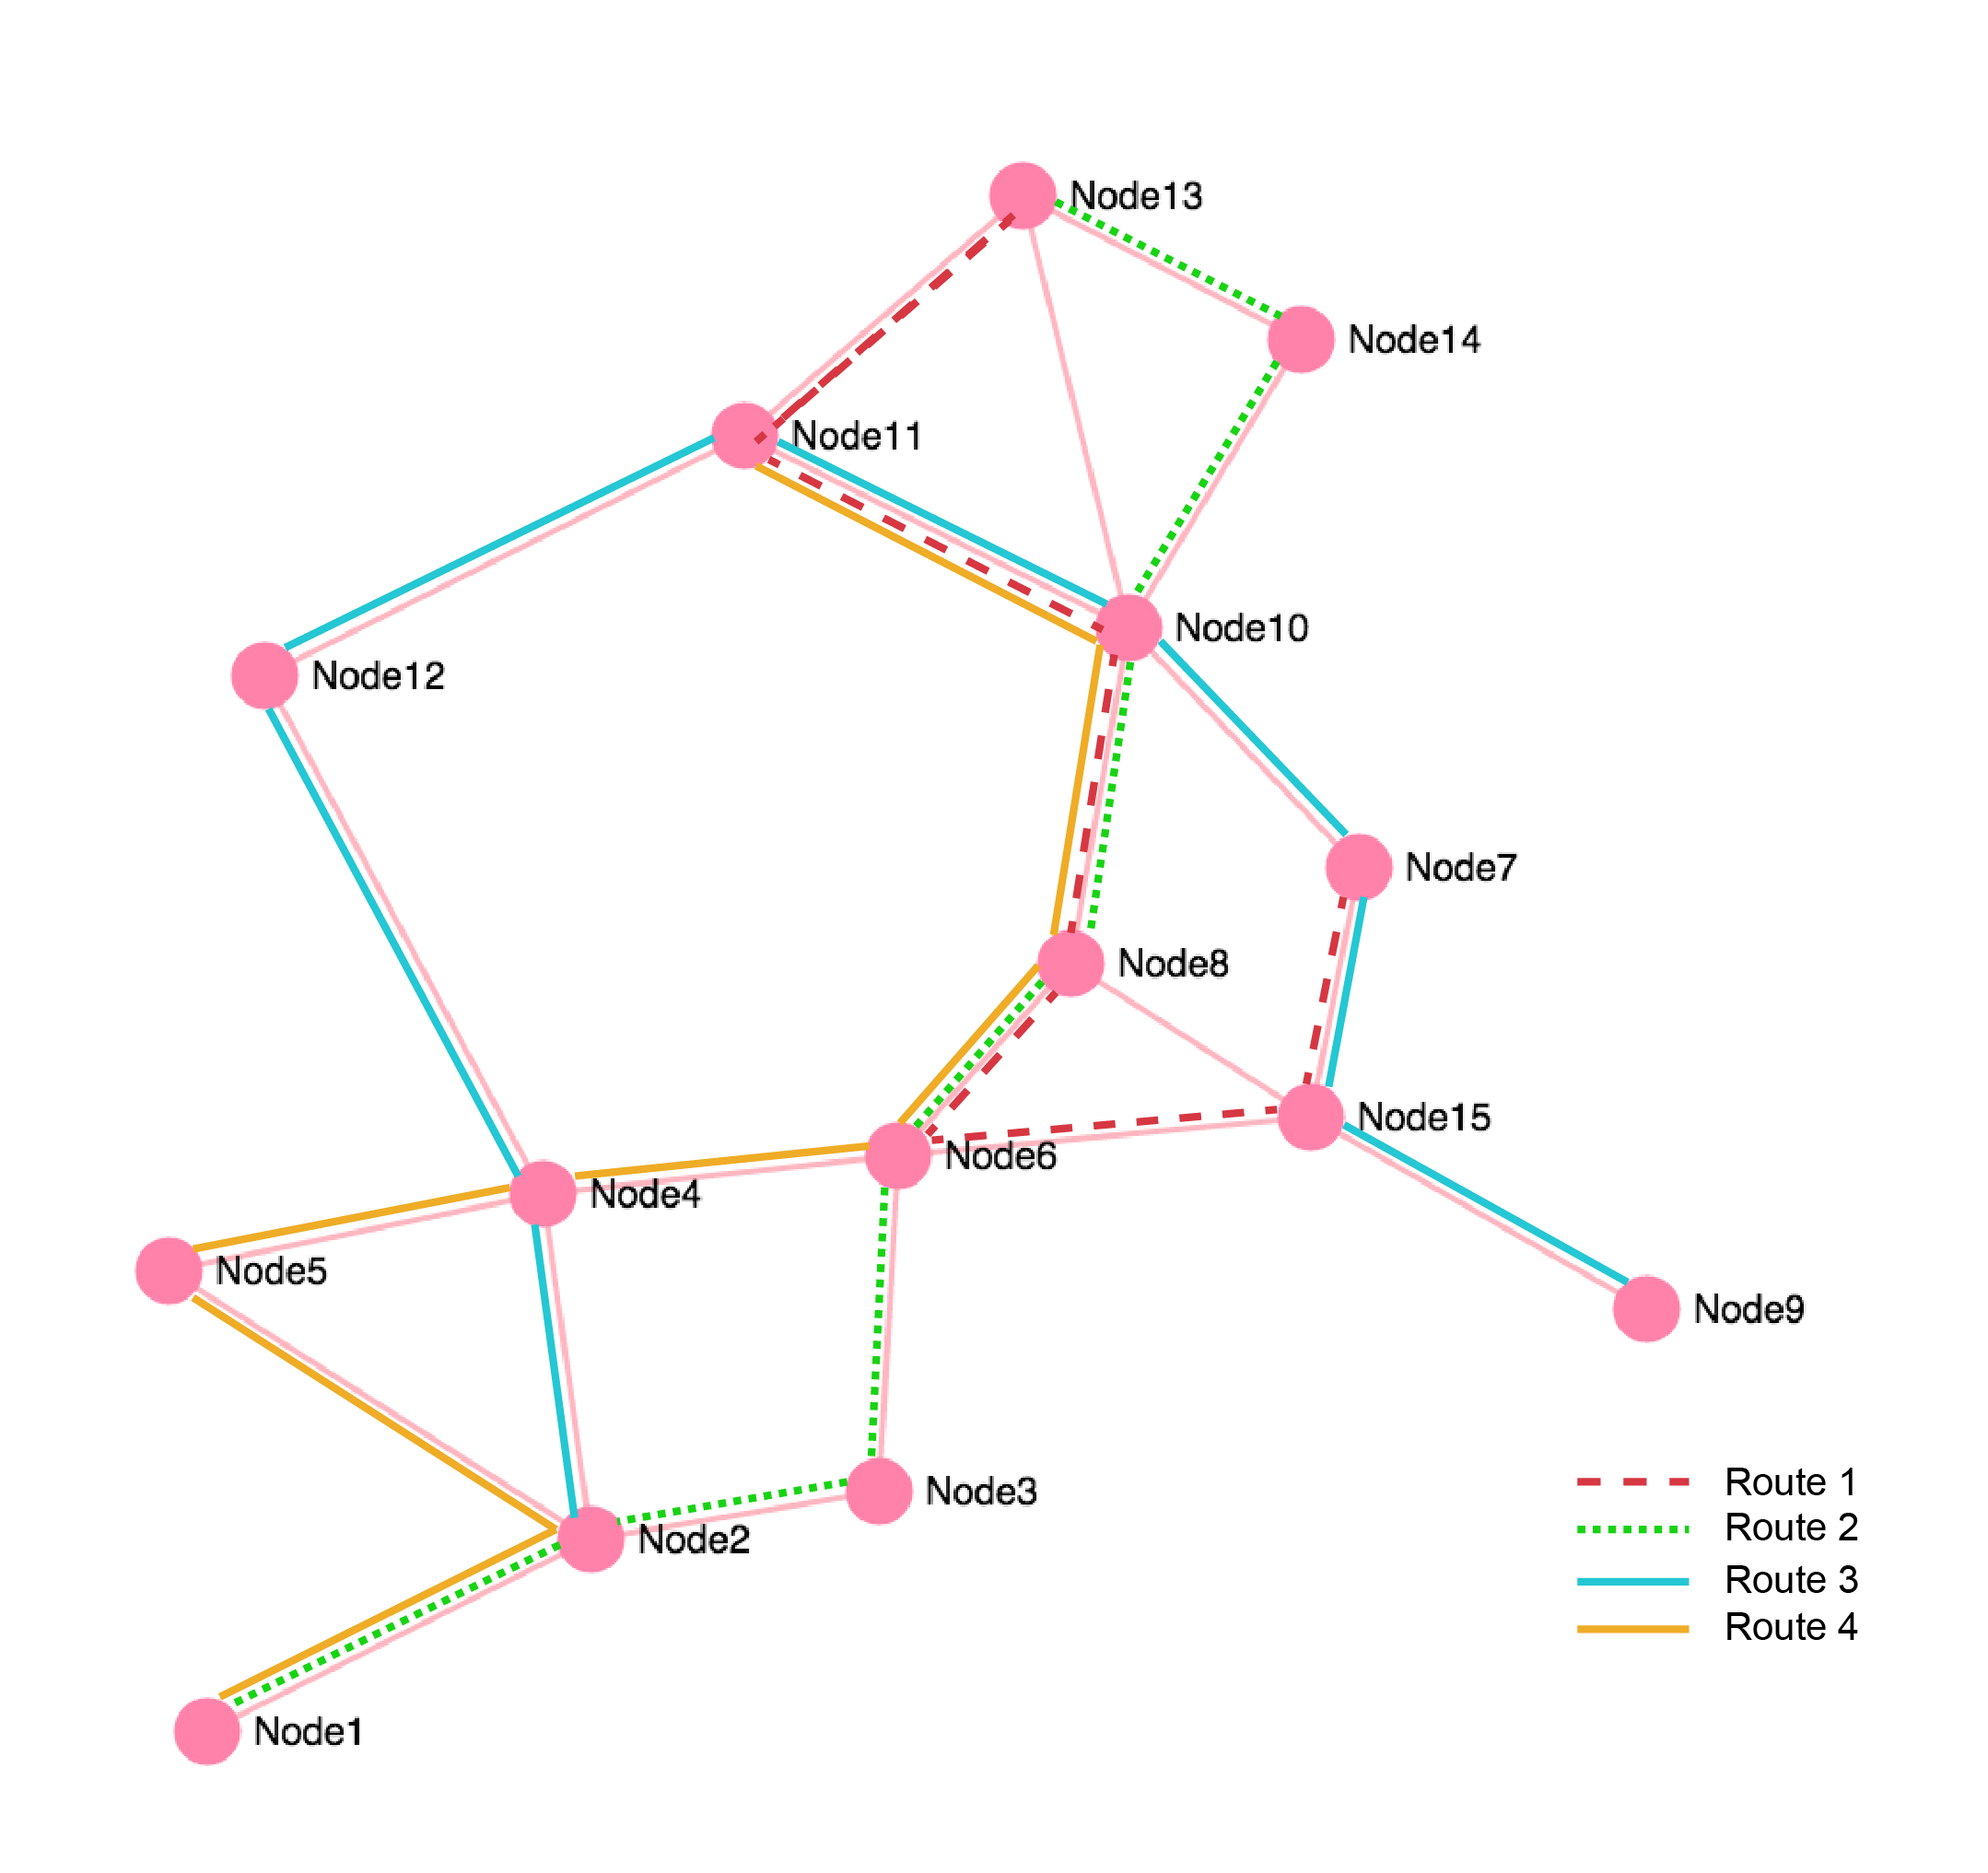
\includegraphics[width=4in]{assets/mandlnetwork_4routes.png}
    \end{center}
    \caption{Illustration of the best route set, having four routes, constructed by the proposed algorithm (Mandl's transit network as a graph)}
    \label{fig:bestRouteSet4} 
\end{figure}

Table \vref{table:performanceComparison_4} presents the results produced by the proposed algorithm (SSO), having four routes, and results from route sets constructed by other approaches.

\begin{table}[H]
	\centering
    \hspace*{-1.0cm}
    \begin{tabular}{|l||l|l|l|l|l|}
 	\hline
 	Algorithm & $d_0(\%)$ & $d_1(\%)$ & $d_2(\%)$ & $d_{unsat}(\%)$ & $ATT$ \\
 	\hline
    \citet{mandl79} & 69.94 & 29.93 & 0.13 & 0.00 & 12.90 \\
    \citet{kechagiopoulos14} avg & 90.52 & 8.75 & 0.73 & 0.00 & 10.71 \\
    \citet{kechagiopoulos14} best & 91.84 & 7.64 & 0.51 & 0.00 & 10.64 \\
    \citet{nikolic14} avg & 95.05 & 4.95 & 0.00 & 0.00 & -$^b$ \\
    \citet{kidwai98} & 72.95 & 26.91 & 0.13 & 0.00 & 12.72 \\
    \citet{fan10} best & 93.26 & 6.74 & 0.00 & 0.00 & 11.37 \\
    \citet{fan10} HC avg & 91.83 & 8.17 & 0.00 & 0.00 & 11.69 \\
    \citet{fan10} SA avg & 92.48 & 7.52 & 0.00 & 0.00 & 11.55 \\
    \citet{chakroborty02} & 86.86 & 12.00 & 1.14 & 0.00 & 11.90 \\
    \citet{zhang10} & 91.46 & 8.54 & 0.00 & 0.00 & 10.65 \\
    \citet{chew12} avg & 92.88 & 6.91 & 0.20 & 0.00 & 11.16 \\
    \citet{chew12} best & 93.71 & 6.29 & 0.00 & 0.00 & 10.82 \\
	\hline
    \hline
    SSO Best & 88.44 & 10.28 & 1.29 & 0.00 & 10.67 \\
    SSO Average & 77.32 & 20.15 & 2.47 & 0.07 & 11.27 \\
    SSO Median & 77.14 & 20.49& 2.25 & 0.00 & 11.26 \\
    SSO Worst & 68.79 & 28.84 & 2.25 & 0.13 & 11.67 \\
    SSO Standard Deviation & 3.91& 3.60 & 1.36 & 0.19 & 0.22 \\
    SSO Relative Standard Deviation & 5.06\% & 17.85\% & 55.16\% & 291.28\% & 1.97\% \\
    %SSO Confidence interval$^b$ & ~ & ~ & ~ & ~ & ~ \\
    \hline
    \end{tabular}
    \caption {Comparing the best route set, having four routes, produced by the proposed algorithm with route sets constructed by other approaches.}
    \begin{itemize}[noitemsep]
    %\item[$^a$:] mintues per user
    \item[$^b$:] 
    %\item[$^b$:] Confidence Interval with a confidence level of 95\%
    \end{itemize}
    \label{table:performanceComparison_4}
\end{table}

%-------------------- 6 route sets ---------------------

    \begin{table}[H]
    \centering
    \begin{tabular}{|l|l l l l l l l l|}
    \hline
    Route 1: & ~ & ~ & ~ & ~ & ~ & ~ & ~ & ~ \\
    Route 2: & ~ & ~ & ~ & ~ & ~ & ~ & ~ & ~ \\
    Route 3: & ~ & ~ & ~ & ~ & ~ & ~ & ~ & ~ \\
    Route 4: & ~ & ~ & ~ & ~ & ~ & ~ & ~ & ~ \\
    Route 5: & ~ & ~ & ~ & ~ & ~ & ~ & ~ & ~ \\
    Route 6: & ~ & ~ & ~ & ~ & ~ & ~ & ~ & ~ \\
    \hline
    \end{tabular}
    \caption {The best route set, having six routes}
    \label{table:performanceComparison_bestRouteSet6}
    \end{table}

    \begin{table}[H]
    \centering
    \hspace*{-1.0cm}
    \begin{tabular}{|l||l|l|l|l|l|}
    \hline
    Algorithm & $d_0(\%)$ & $d_1(\%)$ & $d_2(\%)$ & $d_{unsat}(\%)$ & $ATT$ \\
    \hline
    \citet{kechagiopoulos14} avg & 95.62 & 4.28 & 0.10 & 0.00 & 10.28 \\
    \citet{kechagiopoulos14} best & 96.21 & 3.47 & 0.32 & 0.00 & 10.23 \\
    \citet{nikolic14} & 94.34 & 5.65 & 0.00 & 0.00 & - \\
    \citet{kidwai98} & 77.92 & 19.62 & 2.40 & 0.00 & 10.78 \\
    \citet{fan10} best & 91.52 & 8.48 & 0.00 & 0.00 & 10.48  \\
    \citet{fan10} HA avg & 90.23 & 9.26 & 0.51 & 0.00 & 11.69 \\
    \citet{fan10} SA avg & 90.87 & 8.74 & 0.39 & 0.00 & 10.65 \\
    \citet{chakroborty02} & 86.04 & 13.96 & 0.00 & 0.00 & 10.30 \\
    \citet{zhang10} & 91.12 & 8.88 & 0.00 & 0.00 & 10.50 \\
    \citet{chew12} avg & 93.85 & 5.88 & 0.24 & 0.03 & 10.51 \\
    \citet{chew12} best & 95.57 & 4.43 & 0.00 & 0.00 & 10.28 \\
    \citet{baaj91} & 78.61 & 21.39 & 0.00 & 0.00 & 11.86 \\
    \hline
    \hline
    SSO Best & ~ & ~ & ~ & ~ & ~ \\
    SSO Average & ~ & ~ & ~ & ~ & ~ \\
    SSO Median & ~ & ~ & ~ & ~ & ~ \\
    SSO Worst & ~ & ~ & ~ & ~ & ~ \\
    SSO Standard Deviation & ~ & ~ & ~ & ~ & ~ \\
    SSO Relative Standard Deviation & ~ & ~ & ~ & ~ & ~ \\
    \hline
    \end{tabular}
    \caption {Comparing the best route set, having six routes, produced by the proposed algorithm with route sets constructed by other approaches.}
    \label{table:performanceComparison_6}
    \end{table}

%-------------------- 7 route sets ---------------------

\begin{table}[H]
    \centering
    \begin{tabular}{|l|l l l l l l l l|}
    \hline
    Route 1: & ~ & ~ & ~ & ~ & ~ & ~ & ~ & ~ \\
    Route 2: & ~ & ~ & ~ & ~ & ~ & ~ & ~ & ~ \\
    Route 3: & ~ & ~ & ~ & ~ & ~ & ~ & ~ & ~ \\
    Route 4: & ~ & ~ & ~ & ~ & ~ & ~ & ~ & ~ \\
    Route 5: & ~ & ~ & ~ & ~ & ~ & ~ & ~ & ~ \\
    Route 6: & ~ & ~ & ~ & ~ & ~ & ~ & ~ & ~ \\
    Route 7: & ~ & ~ & ~ & ~ & ~ & ~ & ~ & ~ \\
    \hline
    \end{tabular}
    \caption {The best route set, having seven routes}
    \label{table:performanceComparison_bestRouteSet7}
    \end{table}

    \begin{table}[H]
    \centering
    %\hspace*{-2.0cm}
    \begin{tabular}{|l||l|l|l|l|l|}
    \hline
    Algorithm & $d_0(\%)$ & $d_1(\%)$ & $d_2(\%)$ & $d_{unsat}(\%)$ & $ATT$ \\
    \hline
    \citet{kechagiopoulos14} avg & 96.55 & 3.45 & 0.01 & 0.00 & 10.23 \\
    \citet{kechagiopoulos14} best & 97.17 & 2.83 & 0.00 & 0.00 & 10.16 \\
    \citet{nikolic14} & 94.41 & 5.59 & 0.00 & 0.00 & - \\
    \citet{kidwai98} & 93.91 & 6.09 & 0.00 & 0.00 & 10.70 \\
    \citet{fan10} best & 93.32 & 7.13 & 0.32 & 0.00 & 10.42  \\
    \citet{fan10} HC avg & 92.21 & 7.13 & 0.66 & 0.00 & 10.74 \\
    \citet{fan10} SA avg & 92.47 & 6.95 & 0.58 & 0.00 & 10.62 \\
    \citet{chakroborty02} & 89.15 & 10.85 & 0.00 & 0.00 & 10.15 \\
    \citet{zhang10} & 92.89 & 7.11 & 0.00 & 0.00 & 10.46 \\
    \citet{chew12} avg & 96.47 & 3.53 & 0.00 & 0.00 & 10.31 \\
    \citet{chew12} best & 95.57 & 4.42 & 0.00 & 0.00 & 10.27 \\
    \citet{baaj91} & 80.99 & 19.01 & 0.00 & 0.00 & 12.50 \\
    \hline
    \hline
    SSO Best & ~ & ~ & ~ & ~ & ~ \\
    SSO Average & ~ & ~ & ~ & ~ & ~ \\
    SSO Median & ~ & ~ & ~ & ~ & ~ \\
    SSO Worst & ~ & ~ & ~ & ~ & ~ \\
    SSO Standard Deviation & ~ & ~ & ~ & ~ & ~ \\
    SSO Relative Standard Deviation & ~ & ~ & ~ & ~ & ~ \\
    \hline
    \end{tabular}
    \caption {Comparing the best route set, having seven routes, produced by the proposed algorithm with route sets constructed by other approaches.}
    \label{table:performanceComparison_7}
    \end{table}
%-------------------- 8 route sets ---------------------

\begin{table}[H]
    \centering
    \begin{tabular}{|l|l l l l l l l l|}
    \hline
    Route 1: & ~ & ~ & ~ & ~ & ~ & ~ & ~ & ~ \\
    Route 2: & ~ & ~ & ~ & ~ & ~ & ~ & ~ & ~ \\
    Route 3: & ~ & ~ & ~ & ~ & ~ & ~ & ~ & ~ \\
    Route 4: & ~ & ~ & ~ & ~ & ~ & ~ & ~ & ~ \\
    Route 5: & ~ & ~ & ~ & ~ & ~ & ~ & ~ & ~ \\
    Route 6: & ~ & ~ & ~ & ~ & ~ & ~ & ~ & ~ \\
    Route 7: & ~ & ~ & ~ & ~ & ~ & ~ & ~ & ~ \\
    Route 8: & ~ & ~ & ~ & ~ & ~ & ~ & ~ & ~ \\
    \hline
    \end{tabular}
    \caption {The best route set, having eight routes}
    \label{table:performanceComparison_bestRouteSet8}
    \end{table}

    \begin{table}[H]
    \centering
    \hspace*{-1.0cm}
    \begin{tabular}{|l||l|l|l|l|l|}
    \hline
    Algorithm & $d_0(\%)$ & $d_1(\%)$ & $d_2(\%)$ & $d_{unsat}(\%)$ & $ATT$ \\
    \hline
    \citet{kechagiopoulos14} avg & 97.47 & 2.53 & 0.00 & 0.00 & 10.17 \\
    %Kechapocholous BEST [ref] & 91.84 & 7.64 & 0.51 & 0.00 & 10.64 \\
    \citet{nikolic14} & 96.40 & 3.60 & 0.00 & 0.00 & - \\
    \citet{kidwai98} & 84.73 & 15.27 & 0.00 & 0.00 & 12.22 \\
    %\citet{fan09} best & & & & &  \\
    \citet{fan09} Hill Climbing & 93.23 & 6.18 & 0.59 & 0.00 & 10.69 \\
    \citet{fan09} Simulated Annealing & 93.65 & 5.88 & 0.47 & 0.00 & 10.58 \\
    \citet{chakroborty02} & 90.38 & 9.58 & 0.00 & 0.00 & 10.46 \\
    \citet{zhang10} & 93.14 & 6.86 & 0.00 & 0.00 & 10.42 \\
    \citet{chew12} & 96.16 & 3.84 & 0.00 & 0.09 & 10.31 \\
    \citet{baaj91} & 79.96 & 20.04 & 0.00 & 0.00 & 11.86 \\
    \hline
    \hline
    SSO Best & ~ & ~ & ~ & ~ & ~ \\
    SSO Average & ~ & ~ & ~ & ~ & ~ \\
    SSO Median & ~ & ~ & ~ & ~ & ~ \\
    SSO Worst & ~ & ~ & ~ & ~ & ~ \\
    SSO Standard Deviation & ~ & ~ & ~ & ~ & ~ \\
    SSO Relative Standard Deviation & ~ & ~ & ~ & ~ & ~ \\
    \hline
    \end{tabular}
    \caption {CComparing the best route set, having eight routes, produced by the proposed algorithm with route sets constructed by other approaches.}
    \label{table:performanceComparison_8}
    \end{table}

    %---------------------- Execution time ---------------------
\begin{table}[H]
    \centering
    \begin{tabular}{|l||l|l|l|l|l|l|}
    \hline
    Number of routes & Min & Avg & Median & Max & STD & RSD \\
    \hline
    4 & 491.0 & 555.2 & 553.0 & 644.0 & 31.0 & 5.59\%\\
    \hline
    \end{tabular}
    \caption {Executing time (in seconds) of SSO for route set designs with four, }
   % 100 Monte Carlo runs
    \label{table:performanceComparison_runtime}
    \end{table}




\subsection{Scalability Experiments}
\label{subsec:scalabilityExperiments_results}

\begin{table}[H]
    \centering
    \begin{tabular}{|l|l|l|l|l|l|}
        \hline
        Test case & Nodes&Edges & Method & Running time(sec) \\
        \hline
        1 & 30&90 & 1 & 6764 \\
        \hline
    \end{tabular}
    \caption{Mumford}
    \label{table:results_mumford}
\end{table}
